\sectionbreak \section{  \standartTitleFont
  Модуль DataManipulator
} \label{sec:DataManipulator}

\subsection{ \standartTitleFont
  Назначение модуля DataManipulator
} \label{subsec:targerDM}

{\standartFont

  \par Модуль DataManipulator предназначен для различного рода обработки данных, с целью получения наборов данных (датасетов) необходимых для обучения моделей нейронных сетей. DataManipulator помогает преодолеть этап анализа и обработки данных, а также этап конструирования признаков.

  \par
}

\subsection{ \standartTitleFont
  Главное меню модуля DataManipulator.
} \label{subsec:MainMenuDM}

{\standartFont

  \par В главном меню модуля DataManipulator представлены основные направления для обработки данных. Предоставляется выбор, с каким форматом данных будет происходить работа: с OCDF- или TDF-форматом. В главном меню также можно выбрать пункт, позволяющий создать TDF-данные на основе OCDF-данных. Также имеется пункт, который выводит на экран краткую информацию о форматах данных и о самом модуле DataManipulator. Внешний вид меню можно увидеть на рисунке \ref{fig:mainMenu}

  \par

  \begin{figure}[H]
    \centering
    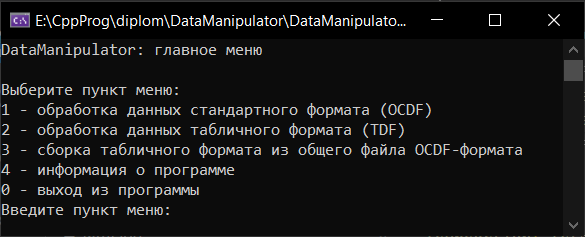
\includegraphics{images/forDataManipulator/mainMenu.png}
    \caption{главное меню модуля DataManipulator}
    \label{fig:mainMenu}
  \end{figure}

}

\subsection{ \standartTitleFont
  Меню обработки данных OCDF-формата модуля DataManipulator.
} \label{subsec:targerDM}

\subsubsection{ \standartTitleFont
  Считывание OCDF-данных из файла.
} \label{subsubsec:ReadOCDF}

{\standartFont

  \par Для того, чтобы попасть в меню по обработке данных OCDF-формата будет предложено для начала их загрузить из файла. Это показано на рисунке на рисунке \ref{fig:readOCDFst1}.

  \begin{figure}[H]
    \centering
    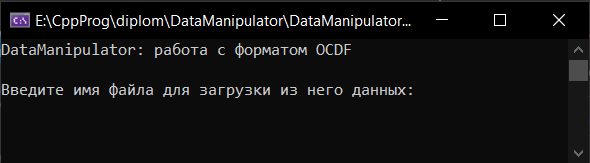
\includegraphics[width=\textwidth]{images/forDataManipulator/readOCDFstage1.png}
    \caption{указание файла для загрузки из него OCDF-данных.}
    \label{fig:readOCDFst1}
  \end{figure}

  \par Вводим путь к файлу или перетаскиваем файл в консоль для получения его абсолютного пути и нажимаем Enter. После этого будет предложено ввести количество данных, которые необходимо считать из файла. Это показано на рисунке \ref{fig:readOCDFst2}.

  \begin{figure}[H]
    \centering
    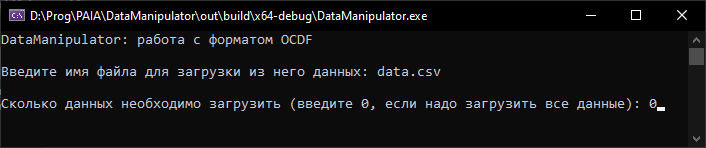
\includegraphics[width=\textwidth]{images/forDataManipulator/readOCDFstage2.png}
    \caption{указание необходимого количества данных для считывания.}
    \label{fig:readOCDFst2}
  \end{figure}

  \par Есть несколько особенностей, при вводе количества данных. В случае, если будет введён 0 или число, превышающее количество данных в файле, то будут считаны все данные, которые есть в файле. Если будет введено отрицательное число или хотя бы один символ, отличный от цифр, то программа выдаст предупреждение о некорректном вводе данных, показанное на рисунке \ref{fig:readOCDFerror1}, и предложит ввести путь к файлу и необходимое количество данных для считывания снова. 

  \begin{figure}[H]
    \centering
    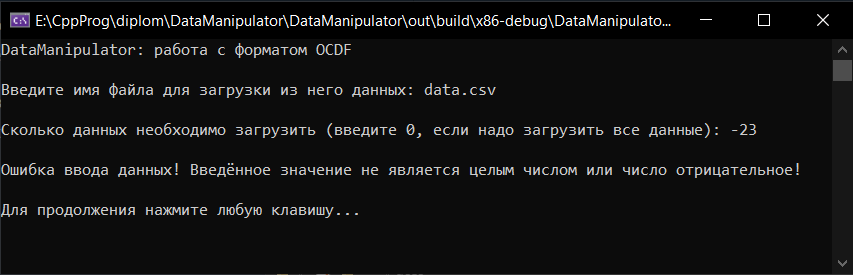
\includegraphics[width=\textwidth]{images/forDataManipulator/readOCDFerror1.png}
    \caption{предупреждение об ошибке при вводе необходимого количества данных для считывания.}
    \label{fig:readOCDFerror1}
  \end{figure}

  \par Могут возникнуть и другие предупреждения, связанные непосредственно с самим файлом. Если файл с данными не существует, или этот файл пуст, или данные в нём не представлены в необходимом формате, то возникнет предупреждение о невозможности чтения данных, представленное на рисунке \ref{fig:readOCDFerror2}.

  \begin{figure}[H]
    \centering
    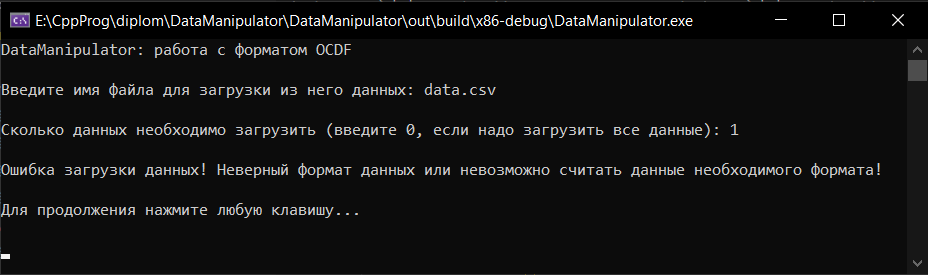
\includegraphics[width=\textwidth]{images/forDataManipulator/readOCDFerror2.png}
    \caption{предупреждение об ошибке чтения данных.} 
    \label{fig:readOCDFerror2}
  \end{figure}

  \par Как уже понятно, чтение данных происходит в текстовом режиме. Однако существует возможность считывать данные, которые представлены в бинарном виде. Для этого необходимо, чтобы файл имел расширение .bin, иначе чтение данных будет происходить в текстовом режиме. Пример файла с данными в бинарном виде можно увидеть на рисунке \ref{fig:readOCDFbin}.

  \begin{figure}[H]
    \centering
    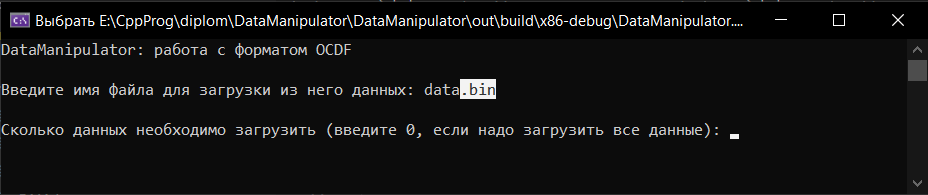
\includegraphics[width=\textwidth]{images/forDataManipulator/readOCDFbin.png}
    \caption{ввод файла с данными в бинарном виде.} 
    \label{fig:readOCDFbin}
  \end{figure}

  \par После указания файла с данными в бинарном виде будет предложено ввести количество данных, которое необходимо считать из файла. Все предупреждения, которые связаны с чтением данных и ввода значений уже разобраны выше. 

  \par
}

\subsubsection{ \standartTitleFont
  Возможности по обработке OCDF-данных. 
} \label{subsubsec:MenuOCDF}

{\standartFont

  \par После считывания OCDF-данных из файла открывается меню для работы с данными, представленное на рисунке \ref{fig:OCDFmenu}.

  \begin{figure}[H]
    \centering
    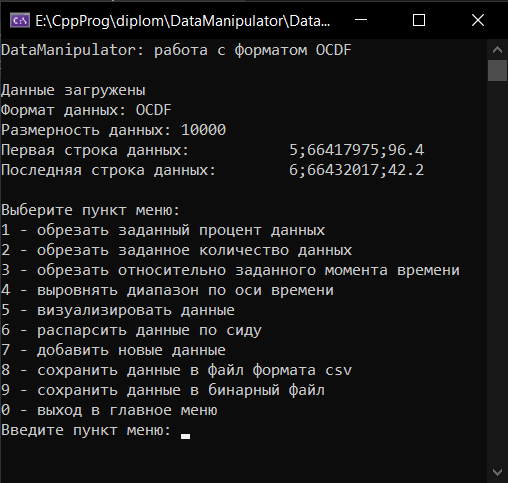
\includegraphics{images/forDataManipulator/OCDFmenu.png}
    \caption{ввод файла с данными в бинарном виде.} 
    \label{fig:OCDFmenu}
  \end{figure}

  \par В появившемся меню будет указана информация о считанных данных: формат данных, их количество, а также первая и последняя строки последовательности данных. После идёт выбор действий, которые можно совершить над данными: обрезка данных, визуализация данных, привидение данных к равноинтервальному виду, парсинг данных, добавление данных и сохранение результатов обработки. Каждое из них подробно будет разобрано ниже.

  \par
}

\subsection{ \standartTitleFont
  Обезка OCDF-данных. 
} \label{subsec:OCDFCut}

{\standartFont

  \par Существует 3 вида обрезки данных: обрезка заданного процента данных, обрезка заданного количества данных и обрезка по заданному моменту времени. Также у каждого вида обрезки данных существует 2 режима обрезки данных: обрезка данных слева направо или обрезка данных справа налево. Рассмотрим каждый вид обрезки данных на примерах данных, показанных на рисунке \ref{fig:ExOCDFdataForCating}. 

  \begin{figure}[H]
    \centering
    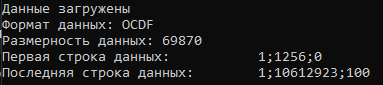
\includegraphics{images/forDataManipulator/ExOCDFdataForCating.png}
    \caption{пример данных для дальнейшей их обрезки.} 
    \label{fig:ExOCDFdataForCating}
  \end{figure}

  \par
}

\subsubsection{ \standartTitleFont
  Обрезка OCDF-данных по заданному проценту. 
} \label{subsubsec:OCDFCutPer}

{\standartFont

  \par Обрезка по заданному проценту данных оставляет введённое пользователем процентное количество данных от общего их количества. Для ввода процента обрезки данных необходимо задать число в промежутке (0,00; 1,00), где 0,00 - 0\%, а 1,00 - 100\%, как это показано на рисунке \ref{fig:OCDFcutper1}. 

  \begin{figure}[H]
    \centering
    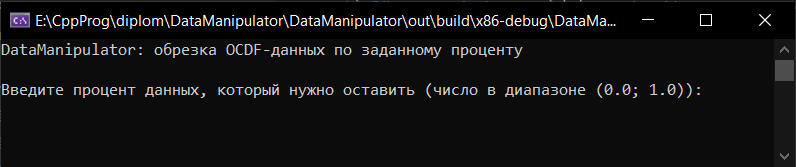
\includegraphics{images/forDataManipulator/OCDFcutpercentstage1.png}
    \caption{ввод процента для обрезки данных.} 
    \label{fig:OCDFcutper1}
  \end{figure}

  \par После ввода процента для обрезки данных, программа предлагает выбрать режим обрезки, введя значения 0 или 1, как показано на рисунке \ref{fig:OCDFcutper2}. 

  \begin{figure}[H]
    \centering
    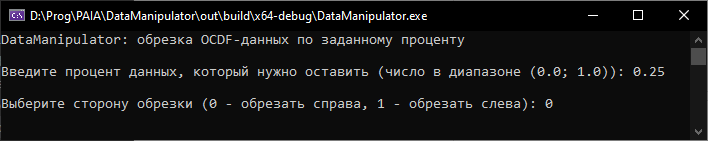
\includegraphics[width=\textwidth]{images/forDataManipulator/OCDFcutpercentstage2.png}
    \caption{ввод режима для обрезки по заданному проценту.} 
    \label{fig:OCDFcutper2}
  \end{figure}

  \par Если ввести 0, то заданный процент данных будет оставлен слева, т.е. в начале. Если ввести 1, то заданный процент данных будет оставлен справа, т.е. в конце. Вводим режим обрезки данных 0 и смотрим результаты на рисунке \ref{fig:ExOCDFdataAftCatPer}. 

  \begin{figure}[H]
    \centering
    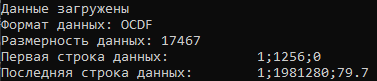
\includegraphics{images/forDataManipulator/ExOCDFdataAftCatPer.png}
    \caption{результаты обрезки данных по заданному проценту.} 
    \label{fig:ExOCDFdataAftCatPer}
  \end{figure}

  \par Была произведена обрезка 75\% данных от общего количества, поскольку было введён 25\% данных, которые необходимо оставить, в режиме справа налево, т.е. с конца. 

  \par 
}

\subsubsection{ \standartTitleFont
  Обрезка OCDF-данных по заданному количеству. 
} \label{subsubsec:OCDFCutQuan}

{\standartFont

  \par Обрезка по заданному количеству данных оставляет введённое пользователем количество данных. Для ввода количества обрезки данных необходимо задать целое положительное число отличное от нуля, как это показано на рисунке \ref{fig:OCDFcutquan1}. 

  \begin{figure}[H]
    \centering
    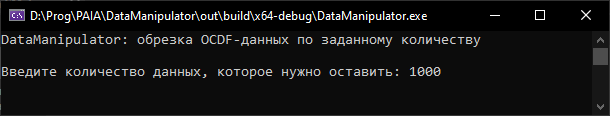
\includegraphics{images/forDataManipulator/OCDFcutquantitystage1.png}
    \caption{ввод значения количества для обрезки данных.} 
    \label{fig:OCDFcutquan1}
  \end{figure}

  \par После ввода количества для обрезки данных, программа предлагает выбрать режим обрезки, введя значения 0 или 1, как показано на рисунке \ref{fig:OCDFcutquan2}. 

  \begin{figure}[H]
    \centering
    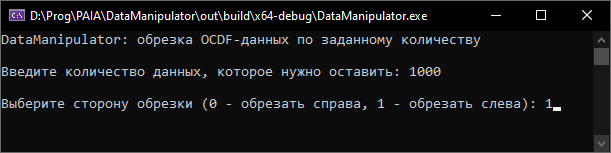
\includegraphics{images/forDataManipulator/OCDFcutquantitystage2.png}
    \caption{ввод режима для обрезки по заданному количеству.} 
    \label{fig:OCDFcutquan2}
  \end{figure}

  \par Если ввести 0, то заданное количество данных будет оставлено слева, т.е. в начале. Если ввести 1, то заданное количество данных будет оставлено справа, т.е. в конце. Вводим режим обрезки данных 1 и смотрим результаты на рисунке \ref{fig:ExOCDFdataAftCatQuan}. 

  \begin{figure}[H]
    \centering
    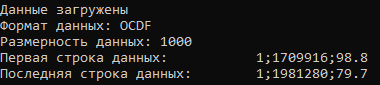
\includegraphics{images/forDataManipulator/ExOCDFdataAftCatQuan.png}
    \caption{результаты обрезки данных по заданному количеству.} 
    \label{fig:ExOCDFdataAftCatQuan}
  \end{figure}

  \par Была произведена обрезка 16467 данных, поскольку было введено 1000 данных, которые необходимо оставить, в режиме справа налево, т.е. в конце. 

  \par 
}

\subsubsection{ \standartTitleFont
  Обрезка OCDF-данных по заданному моменту времени. 
} \label{subsubsec:OCDFCutMom}

{\standartFont

  \par Обрезка по заданному моменту времени оставляет промежуток данных до или после указанного момента. Для ввода момента времени для обрезки данных необходимо задать целое положительное число отличное от нуля, как это показано на рисунке \ref{fig:OCDFcutmom1}. 

  \begin{figure}[H]
    \centering
    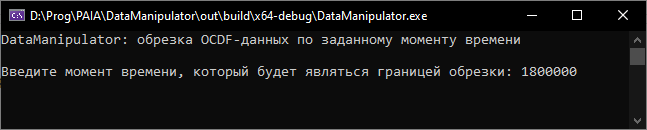
\includegraphics{images/forDataManipulator/OCDFcutmomentstage1.png}
    \caption{ввод значения момента времени для обрезки данных.} 
    \label{fig:OCDFcutmom1}
  \end{figure}

  \par После ввода момента времени для обрезки данных, программа предлагает выбрать режим обрезки, введя значения 0 или 1, как показано на рисунке \ref{fig:OCDFcutmom2}. 

  \begin{figure}[H]
    \centering
    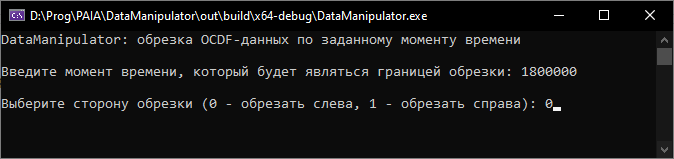
\includegraphics[width=\textwidth]{images/forDataManipulator/OCDFcutmomentstage2.png}
    \caption{ввод режима для обрезки по заданному моменту времени.} 
    \label{fig:OCDFcutmom2}
  \end{figure}

  \par Если ввести 0, то данные будут оставлены слева относительно заданного момента времени, т.е. в начале. Если ввести 1, то данные будут оставлены справа относительно заданного момента времени, т.е. в конце. Вводим режим обрезки данных 0 и смотрим результаты на рисунке \ref{fig:ExOCDFdataAftCatMom}. 

  \begin{figure}[H]
    \centering
    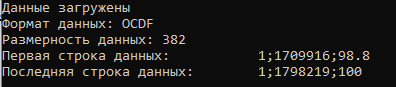
\includegraphics{images/forDataManipulator/ExOCDFdataAftCatMom.png}
    \caption{результаты обрезки данных по заданному моменту времени времени.} 
    \label{fig:ExOCDFdataAftCatMom}
  \end{figure}

  \par 
}

\subsubsection{ \standartTitleFont
  Возможные ошибки при обрезке OCDF-данных. 
} \label{subsubsec:OCDFCutErr}

{\standartFont

  \par При обрезке данных могут возникать различные ситуации, которые способны вызывать всяческие ошибки или исключительные случаи. Самым основным, что может вызвать ошибку, это некорректный ввод данных. Так, например, при обрезке данных по заданному проценту не допустимо вводить числа, не принадлежащие диапазону (0,00; 1,00), хоть и ввод 1,00 доступен, однако при этом данные никак не изменятся. Ввод отрицательных или не целых чисел при обрезке по заданному моменту времени и по заданному количеству данных также вызывает ошибки некорректного ввода. Пример такой ошибки продемонстрирован на рисунке \ref{fig:ExOCDFdataCatErr1}.

  \begin{figure}[H]
    \centering
    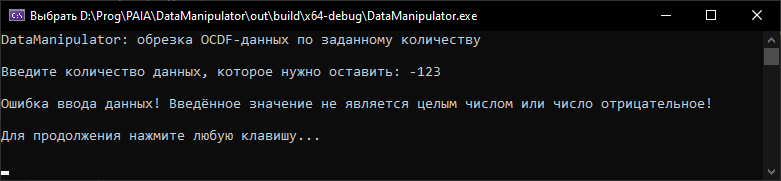
\includegraphics[width=\textwidth]{images/forDataManipulator/ExOCDFdataCatError1.png}
    \caption{пример ввода недопустимых чисел при обрезке OCDF-данных.} 
    \label{fig:ExOCDFdataCatErr1}
  \end{figure}

  \par Также может быть вызвана ошибка некорректного ввода, при использовании символов, отличных от цифр, характерное для всех видов обрезки. Пример такой ошибки продемонстрирован на рисунке \ref{fig:ExOCDFdataCatErr2}.

  \begin{figure}[H]
    \centering
    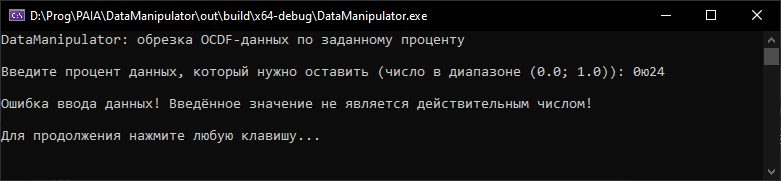
\includegraphics[width=\textwidth]{images/forDataManipulator/ExOCDFdataCatError2.png}
    \caption{пример ввода недопустимых символов при обрезке OCDF-данных.} 
    \label{fig:ExOCDFdataCatErr2}
  \end{figure}

  \par При обрезке данных по заданному количеству есть вероятность того, что пользователь введёт число больше общего количества данных. В таком случае данные не изменятся и ошибка не появится. 

  \par При обрезке данных по заданному моменту времени есть вероятность того, что пользователь введёт момент времени, который находится раньше начального момента времени или позже конечного момента времени в самих данных. В таком случае, если будет выбран соответствующий режим обрезки, данные либо никак не изменятся, либо появится ошибка о возврате пустых данных, что продемонстрирована на рисунке \ref{fig:ExOCDFdataCatErr3}.

  \begin{figure}[H]
    \centering
    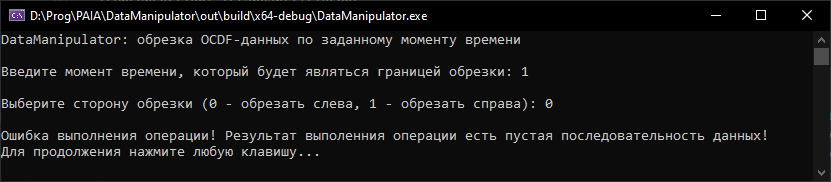
\includegraphics[width=\textwidth]{images/forDataManipulator/ExOCDFdataCatError3.png}
    \caption{пример ошибки при возврате пустых OCDF-данных.} 
    \label{fig:ExOCDFdataCatErr3}
  \end{figure}

  \par Такая ошибка может возникать также при вводе 0,00 для обрезки данных по заданному проценту. В случае такой ошибки данные никак не изменятся и управление перейдёт к меню обработки OCDF-данных.
  
  \par Последняя возможная ошибка относится к вводу недопустимых символов при выборе режимов обрезки. В таком случае возникает ошибка, которая перезапускает операцию заново. Пример такой ошибки продемонстрирован на рисунке \ref{fig:ExOCDFdataCatErr4}.

  \begin{figure}[H]
    \centering
    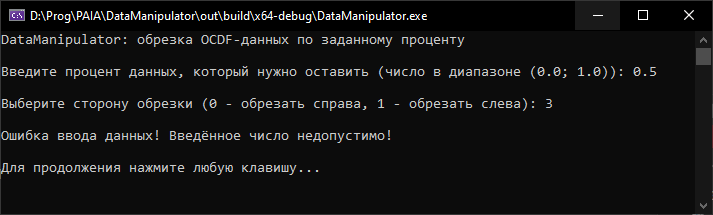
\includegraphics[width=\textwidth]{images/forDataManipulator/ExOCDFdataCatError4.png}
    \caption{пример ввода некорретных данных при выборе режима обрезки OCDF-данных.} 
    \label{fig:ExOCDFdataCatErr4}
  \end{figure}

  \par
}

\subsection{ \standartTitleFont
  Парсинг OCDF-данных. 
} \label{subsec:OCDFPars}

{\standartFont

  \par Основной функцией парсинга данных является разделение данных относительно указанного сида для данных, где имеются значения двух и более сидов, с целью получения данных, содержащих информацию, относящуюся исключительно к указанному сиду.

  \par 
}

\subsubsection{ \standartTitleFont
  Процесс парсинга OCDF-данных. 
} \label{subsubsec:OCDFParsProc}

{\standartFont

  \par Процесс парсинга начинается с того, что программа запрашивает: данные какого сида необходимо получить? Это можно увидеть на рисунке \ref{fig:OCDFdataParsSt}.

  \begin{figure}[H]
    \centering
    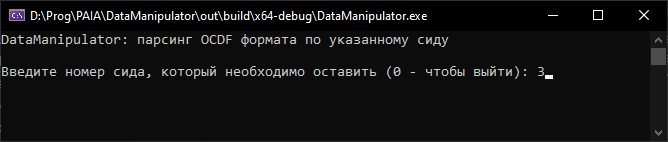
\includegraphics[width=\textwidth]{images/forDataManipulator/OCDFdataParcing.png}
    \caption{ввод номера сида для парсинга OCDF-данных.} 
    \label{fig:OCDFdataParsSt}
  \end{figure}

  \par После ввода номера сида, который необходимо получить, выполняется сам процесс парсинга, результатом которого являются данные, содержащие информацию, касающиеся указанного сида. Данная операция весьма проста.

  \par 
}

\subsubsection{ \standartTitleFont
  Возможные ошибки при парсинге OCDF-данных.
} \label{subsubsec:OCDFParsErr}

{\standartFont

  \par Несмотря на простоту операции парсинга, всей же есть ситуации, при которых возникают ошибки или исключительные случаи. 

  \par Ошибка может возникать, если ввести недопустимый сид. На данный момент программа считает допустимыми следующие сиды: 1, 2, 3, 4, 5, 6. Иные введённые числа вызывают ошибку, продемонстрированную на рисунке \ref{fig:OCDFdataParsErrUnkcid}.

  \begin{figure}[H]
    \centering
    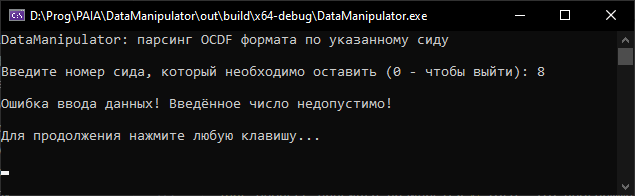
\includegraphics{images/forDataManipulator/OCDFdataParsErrUnknowCID.png}
    \caption{ошибка ввода несуществующего сида при парсинге OCDF-данных.} 
    \label{fig:OCDFdataParsErrUnkcid}
  \end{figure}

  \par Ошибка также может возникать, если ввести недопустимые символы, т.е. символы отличные от цифр. Данная ошибка продемонстрирована на рисунке \ref{fig:OCDFdataParsErrInv}.

  \begin{figure}[H]
    \centering
    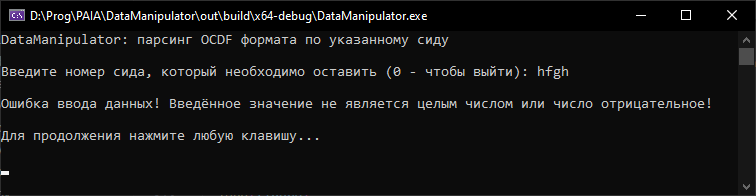
\includegraphics[width=\textwidth]{images/forDataManipulator/OCDFdataParsErrInvalid.png}
    \caption{ошибка ввода недопустимого символа при парсинге OCDF-данных.} 
    \label{fig:OCDFdataParsErrInv}
  \end{figure}

  \par Также ошибка может возникать в случае, если был введён сид, которого нет в данных, подвергаемых парсингу. Данная ошибка продемонстрирована на рисунке \ref{fig:OCDFdataParsErrnotcid}.

  \begin{figure}[H]
    \centering
    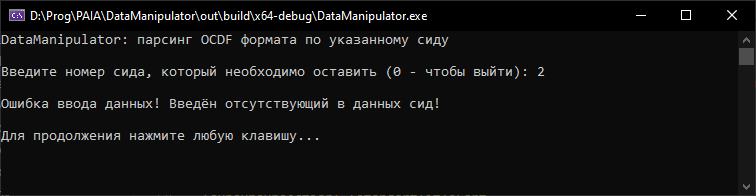
\includegraphics[width=\textwidth]{images/forDataManipulator/OCDFdataParsErrNotCID.png}
    \caption{ошибка ввода отсутствующего сида в OCDF-данных.} 
    \label{fig:OCDFdataParsErrnotcid}
  \end{figure}

  \par Результатом выше перечисленных ошибок будет перезапуск операции парсинга. 

}

\subsection{ \standartTitleFont
  Выравнивание диапазонов OCDF-данных.
} \label{subsec:OCDFRightIntervals}

{\standartFont

  \par Выравнивание диапазонов OCDF-данных по оси времени предполагает формирование равноинтервальных данных. Такие данные необходимы прежде всего для корректной работы модели, чтобы она могла предсказывать поведение графика в определённых моментах времени, иначе точность модели упадёт или возникнут трудности в определении моментов времени у предсказанных величин. 

  \par 
}

\subsubsection{ \standartTitleFont
  Математические основы выравнивания диапазонов OCDF-данных.
} \label{subsubsec:OCDFRIMath}

{\standartFont

  \par Равноинтервальные данные предполагают то, что расстояние или интервалы между соседними точками по оси абсцисс или по оси времени будут взаимо равноудалёнными друг от друга. В таком случае, момент времени каждой точки можно выразить с помощью арифметической прогрессии по формуле \ref{eq:ArefProg}.

  \begin{equation} \label{eq:ArefProg}
    t_i = t_0 + i \cdot r
  \end{equation}

  \begin{tabular}{p{0,4cm}p{15,6cm}}
		где  & $t_0$ {--} начальное значение времени; \\
		 	   & $r$ {--} необходимое расстояние между точками, представляющее собой некоторую константу, которую может задать пользователь; \\
     	   & $i$ {--} номер точки, итерации, элемента прогрессии; $t_i$ {--} i-ит элемент прогрессии;  \\
     	   & $t_i$ {--} i-ит элемент прогрессии. \\
  \end{tabular}

  \par Теперь необходимо определить значение ординаты для каждого нового рассчитанного момента времени. Для этого используем уравнение из аналитической геометрии, а именно уравнение прямой, проходящей через две точки, которое можно увидеть на формуле \ref{eq:AnGeom}.

  \begin{equation} \label{eq:AnGeom}
    \frac{x - x_1}{x_2 - x_1} = \frac{y - y_1}{y_2 - y_1}
  \end{equation}

  \begin{tabular}{p{0,4cm}p{15,6cm}}
    где  & точка $\left(x, y\right)$ {--} это точка, которую необходимо найти между точками $\left(x_1, y_1\right)$ и $\left(x_2, y_2\right)$, взятых из реальных данных. \\
  \end{tabular}

  \par Про соотношение этих точек известно, что $x_1 \leq x \leq x_2$.

  \par Для определение ординаты i-того элемента прогрессии необходимо взять две ближайших точки из реальных данных относительно оси абсцисс к искомой точке. Тогда для определения ординаты имеем формулу \ref{eq:ResRIn}.

  \begin{equation} \label{eq:ResRIn}
    y = \left(\frac{\left(x - x_1\right) \cdot \left(y_2 - y_1\right)}{x_2 - x_1}\right) + y_1
  \end{equation}

  \par Таким образом, можно получить аппроксимированные данные, где взаимное удаление между двумя соседними точками будет везде во всей цепочке данных постоянным.  

  \par 
}

\subsubsection{ \standartTitleFont
  Процесс выравнивания диапазонов OCDF-данных.
} \label{subsubsec:OCDFRIProc}

{\standartFont

  \par Для получения равноинтервальных OCDF-данных необходимо выбрать соответствующий пункт меню, после чего нас встретить сообщение, запрашивающее задать: каким будет интервал между точками? Это продемонстрировано на рисунке \ref{fig:OCDFappr}.

  \begin{figure}[H]
    \centering
    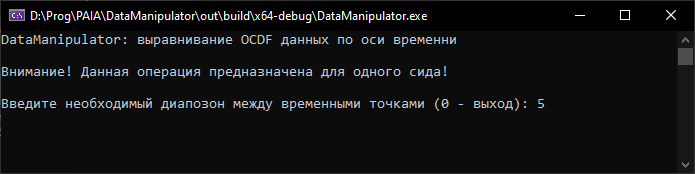
\includegraphics[width=\textwidth]{images/forDataManipulator/OCDFrightIntervals.png}
    \caption{ввод интервала для аппроксимации OCDF-данных.} 
    \label{fig:OCDFappr}
  \end{figure}

  \par Также на рисунке присутствует важное предупреждение, говорящее о том, что данная операция предназначенная для данных, содержащих информацию всего по одному сиду.

  \par После ввода начнётся процесс аппроксимации, в результате которого можно будет получить данные, расстояние между соседними точками которых равно введённому пользователем числу.  

  \par 
}

\subsubsection{ \standartTitleFont
  Возможные ошибки при выравнивании диапазонов OCDF-данных.
} \label{subsubsec:OCDFRIErr}

{\standartFont

  \par Также к знакомой нам уже ошибке относится и ввод отрицательных, не целых чисел и ввод отличных от цифр символов, продемонстрированный на рисунке \ref{fig:OCDFapprerr1}.

  \begin{figure}[H]
    \centering
    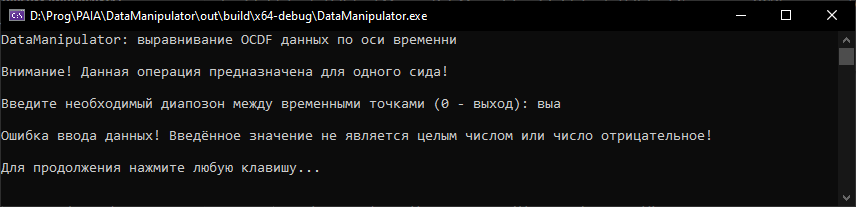
\includegraphics[width=\textwidth]{images/forDataManipulator/OCDFApprErr1.png}
    \caption{ввод некорректных значений при аппроксимации OCDF-данных.} 
    \label{fig:OCDFapprerr1}
  \end{figure}

  \par По сути, при вводе будущего интервала нет никаких ограничений, однако при вводе больших чисел результат может быть неудовлетворительным. Этот момент остаётся на совести пользователя. 

  \par 
}

\subsection{ \standartTitleFont
  Добавление OCDF-данных.
} \label{subsec:OCDFAddData}

{\standartFont

  \par Имеется возможность добавление OCDF-данных к другим OCDF-данным. Это делается с помощью выбора соответствующего пункта меню. Для начала будет предложено ввести имя файла с данными, которые необходимо добавить. Это продемонстрировано на рисунке \ref{fig:AddOCDF}.

  \begin{figure}[H]
    \centering
    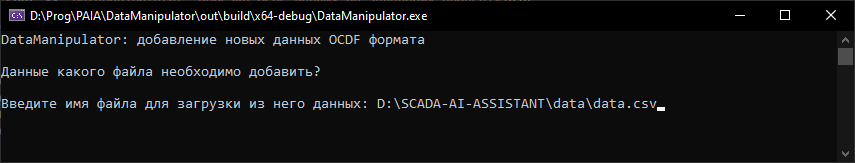
\includegraphics[width=\textwidth]{images/forDataManipulator/AddOCDF.png}
    \caption{ввод файла для добавления OCDF-данных.} 
    \label{fig:AddOCDF}
  \end{figure}

  \par Далее будет предложено ввести количество данных, которых необходимо добавить. Это продемонстрировано на рисунке \ref{fig:AddOCDFHowMany}.
  
  \begin{figure}[H]
    \centering
    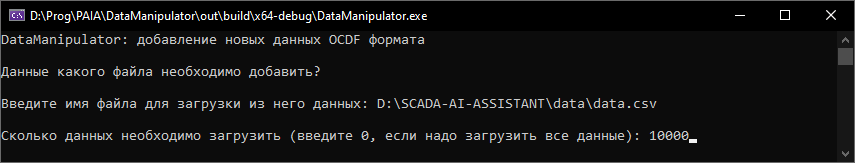
\includegraphics[width=\textwidth]{images/forDataManipulator/AddOCDFHowMany.png}
    \caption{ввод количества OCDF-данных для добавления к другим OCDF-данных.} 
    \label{fig:AddOCDFHowMany}
  \end{figure}

  \par Стоит предупредить, что программа никак не обрабатывает добавляемые данные, за исключением идентификации данных в файле как OCDF, поэтому добавление новых данных ложится на совесть пользователя. Он должен знать, что он добавляет, иначе операция может пройти корректно, но, например, одни данные могут быть равноинтервальными, а другие нет, разрыв, расстояние между добавленными и исходными данными может быть огромным и так далее. 

  \par Впрочем, при добавлении данных, новые и старые данные смешиваются и сортируются по хронологическому порядку. Стоит отметить также и то, что данная функция может нарушать основное правило временных рядов: все данные отсортированы в хронологическом порядке и нет данных с одинаковым временным моментом. Нарушается скорее вторая часть правила. При добавлении данных могут быть значения, относящиеся к моментам времени, которые уже определены в исходных данных. В таком случае данные всё равно добавятся. В одном временном моменте сначала будут идти исходные данные, а затем только добавленные. 

  \par К ошибкам во время процесса добавления можно отнести ошибки, описанные в разделе \ref{subsubsec:ReadOCDF}.

  \par 
}

\subsection{ \standartTitleFont
  Визуализация OCDF-данных.
} \label{subsubsec:OCDFVisual}

{\standartFont

  \par Для визуализации OCDF-данных достаточно выбрать соответствующий пункт меню и дождаться появления окна с визуализированными данными. Вводить ничего не требуется. 

  \par Визуализация данных может проходить по-разному. Всё зависит от данных, которые требуется визуализировать. Если в данных содержится информация, касаемая исключительно одного сида, то в окне визуализации появится только один график, а оси будут подписаны в соответствии с тем, что обозначает визуализированный сид. Это можно увидеть на рисунке \ref{fig:OCDFVisualOneCID}.

  \begin{figure}[H]
    \centering
    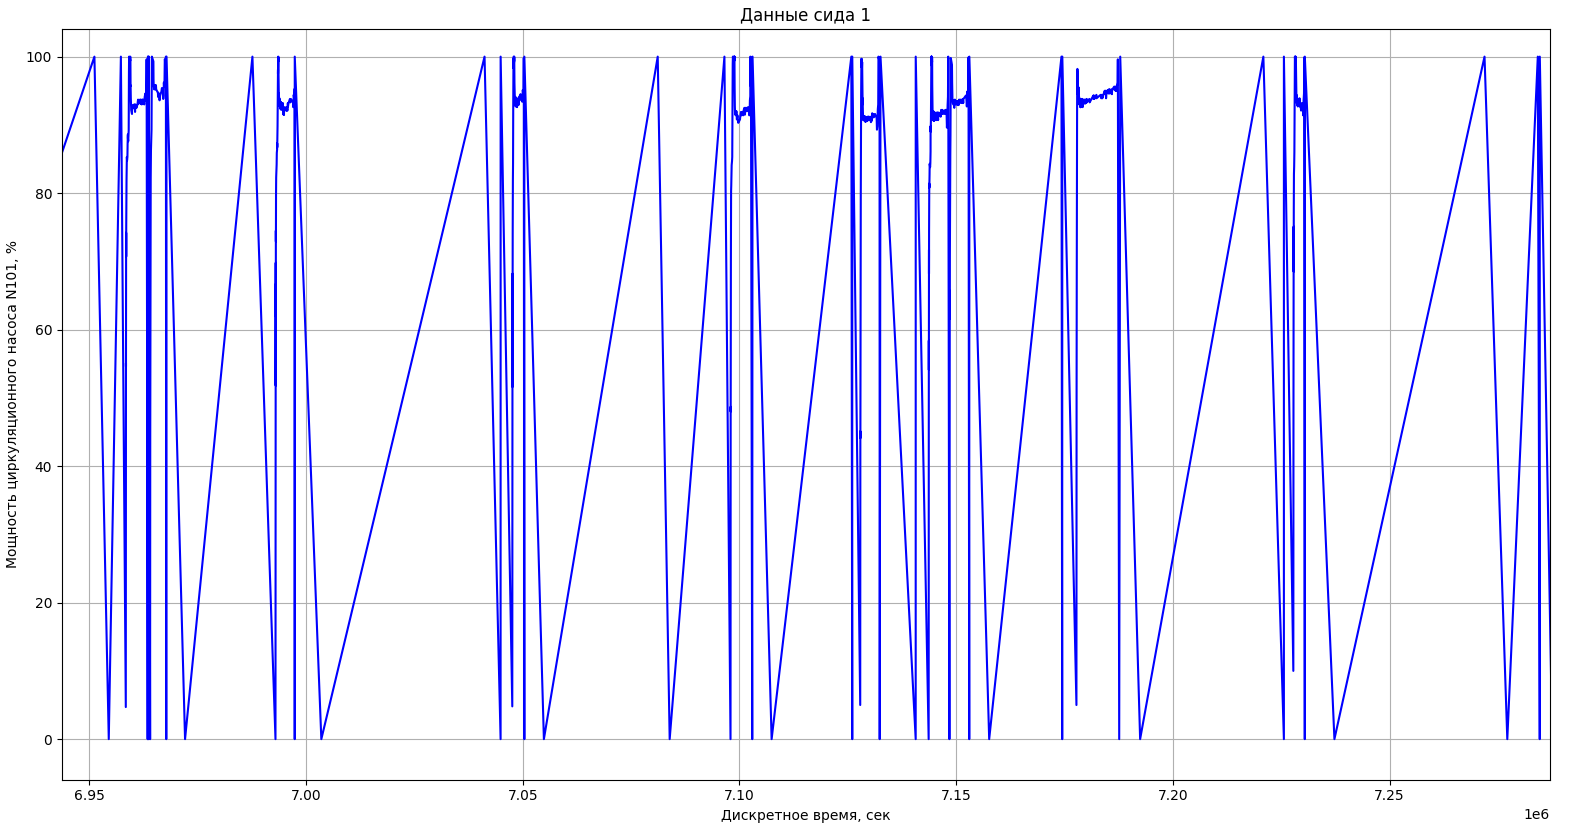
\includegraphics[width=\textwidth]{images/forDataManipulator/OCDFVisualOneCID.png}
    \caption{визуализация OCDF-данных одного сида} 
    \label{fig:OCDFVisualOneCID}
  \end{figure}

  \par В случае, если данные содержат информацию более одно сида, то во-первых будет построено столько графиков, сколько сидов содержится в данных, во-вторых, появится легенда, дающая информацию о визуализированных сидах, в-третьих ось ординат не будет никак подписана, вся информация хранится в легенде. Это можно увидеть на рисунках \ref{fig:OCDFVisualTwoCIDs} и \ref{fig:OCDFVisualAllCIDs}.

  \begin{figure}[H]
    \centering
    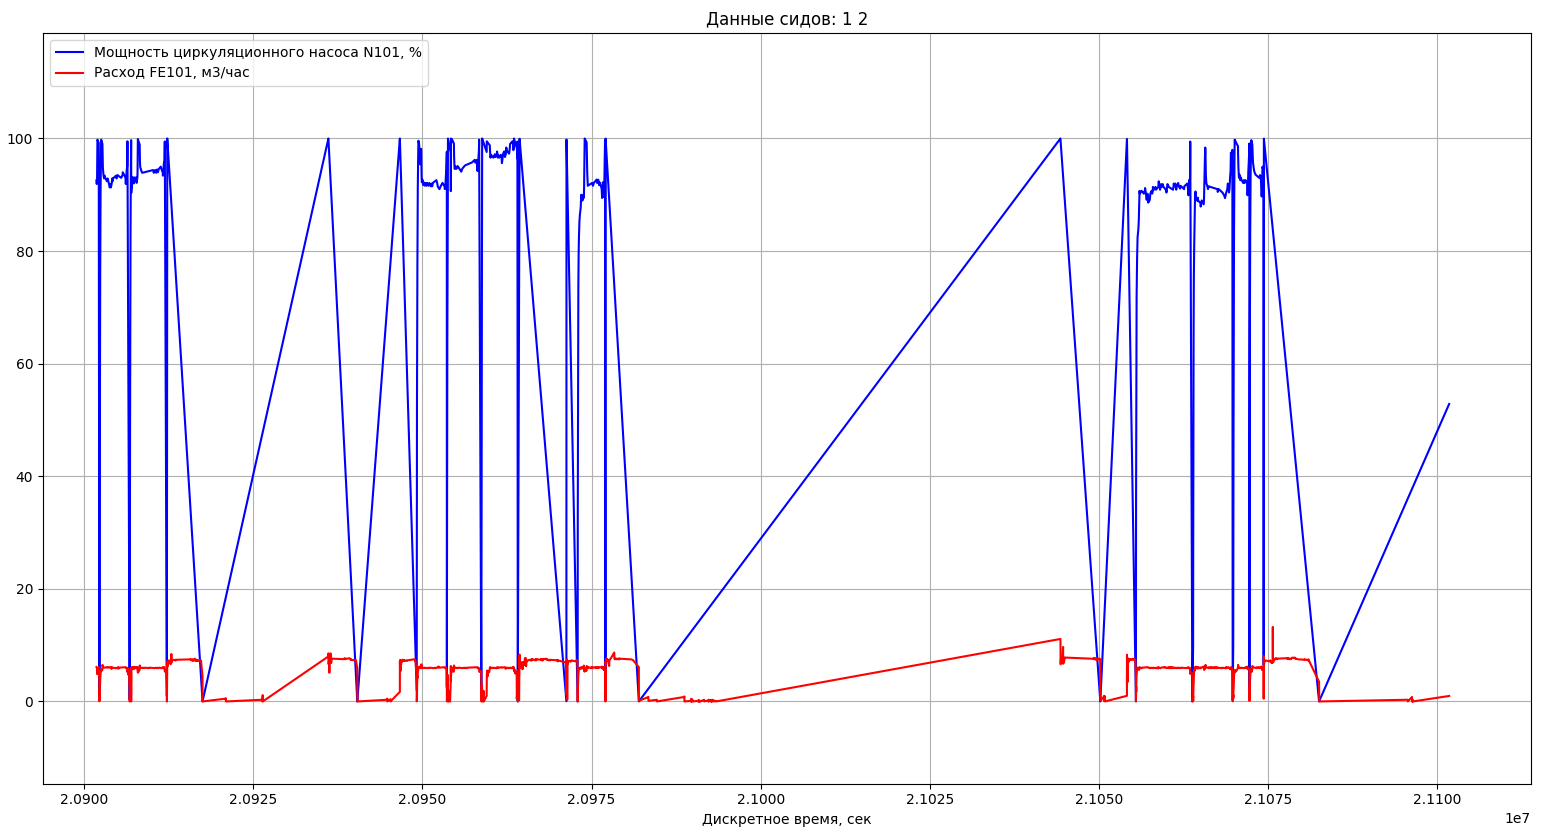
\includegraphics[width=\textwidth]{images/forDataManipulator/OCDFVisualTwoCIDs.png}
    \caption{пример визуализация OCDF-данных с двумя сидами} 
    \label{fig:OCDFVisualTwoCIDs}
  \end{figure}

  \begin{figure}[H]
    \centering
    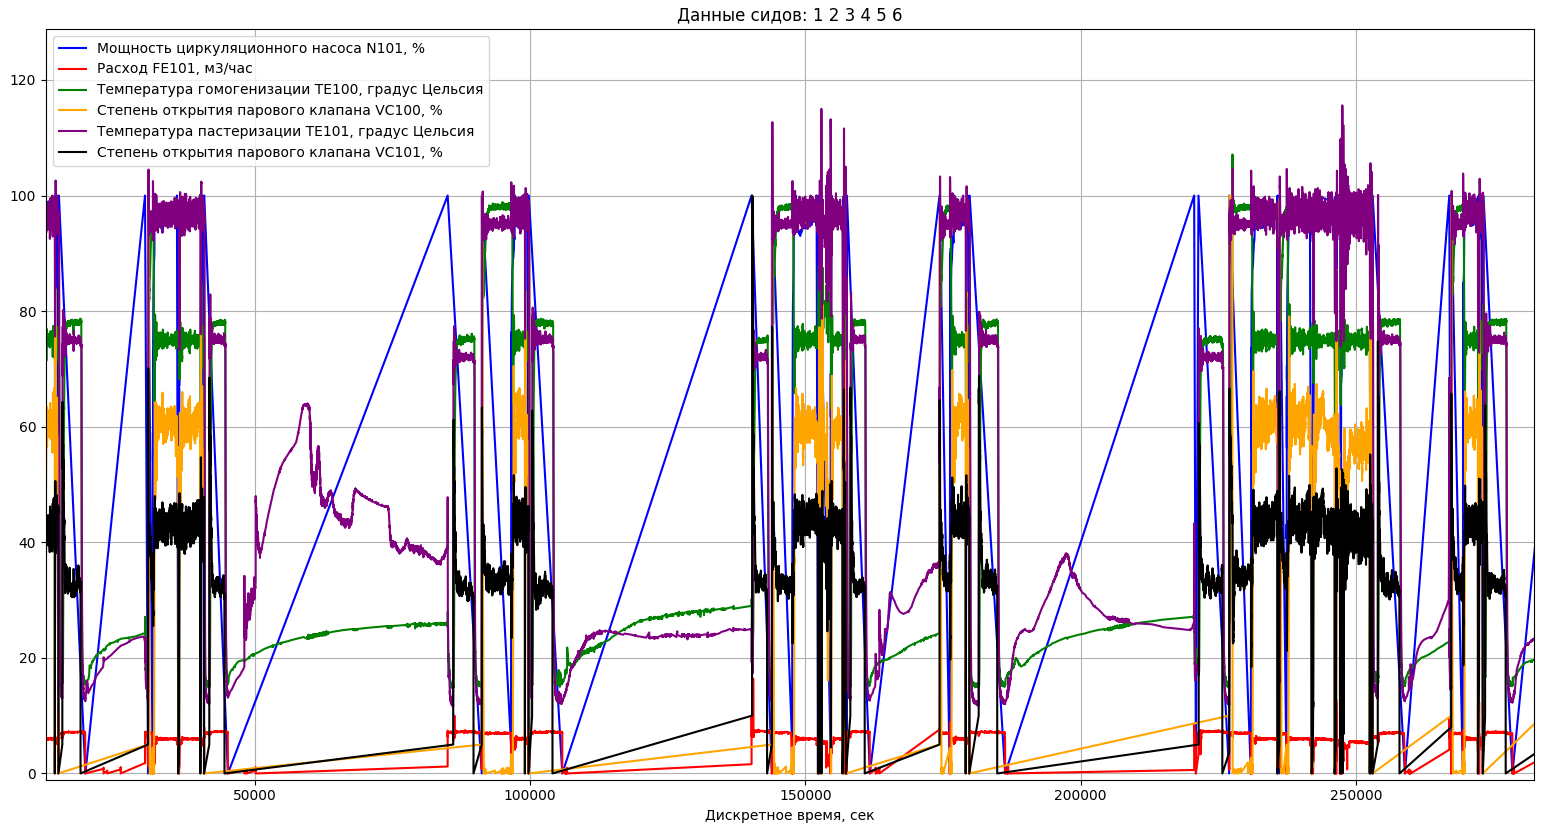
\includegraphics[width=\textwidth]{images/forDataManipulator/OCDFVisualAllCIDs.png}
    \caption{пример визуализация OCDF-данных со всеми сидами}
    \label{fig:OCDFVisualAllCIDs}
  \end{figure}

  \par Управление перейдёт к основной программе только после закрытия окна визуализации.  

  \par 
}

\subsubsection{ \standartTitleFont
  Управление визуализацией OCDF-данных.
} \label{subsubsec:OCDFVisualControl}


{\standartFont

  \par При визуализации данных предусмотрено масштабирование окна визуализации. Прежде чем об этом рассказать, определить два сокращения. Первое сокращение: вращение колёсика мышки вперёд (от себя) {--} вкмВ. Второе сокращение: вращение колёсика мышки назад (на себя) {--} вкмН. Тогда имеем:

  \par вкмВ {--} позволяет увеличить масштаб окна визуализации. Проще говоря, позволяет приблизить изображение.

  \par вкмН {--} позволяет уменьшить масштаб окна визуализации. Проще говоря, позволяет отдалить изображение.

  \par Shift + вкмВ {--} позволяет увеличить масштаб по оси абсцисс (оси времени, оси X, нижней оси) окна визуализации. Проще говоря, позволяет растянуть изображение по ширине.

  \par Shift + вкмН {--} позволяет уменьшить масштаб по оси абсцисс (оси времени, оси X, нижней оси) окна визуализации. Проще говоря, позволяет сжать изображение по ширине.

  \par CTRL + вкмВ {--} позволяет увеличить масштаб по оси ординат (оси значений, оси У, боковой оси) окна визуализации. Проще говоря, позволяет растянуть изображение по высоте.

  \par CTRL + вкмН {--} позволяет уменьшить масштаб по оси ординат (оси значений, оси У, боковой оси) окна визуализации. Проще говоря, позволяет сжать изображение по высоте.

  \par
}

\subsection{ \standartTitleFont
  Сохранение OCDF-данных в файл.
} \label{subsubsec:OCDFSafe}

{\standartFont

  \par После работы с данными конечно же появится надобность в сохранении результатов обработки данных. Для этого есть возможность сохранить данные в текстовом или бинарном режимах. 

  \par 
}

\subsubsection{ \standartTitleFont
  Сохранение OCDF-данных в файл формата csv.
} \label{subsubsec:OCDFSafeCSV}

{\standartFont

  \par Для сохранения данных в текстовом режиме нужно выбрать соответствующий пункт меню и в появившемся запросе указать путь к файлу, в который будут сохранены данные. Это продемонстрировано на рисунке \ref{fig:OCDFsafeCSV}.

  \begin{figure}[H]
    \centering
    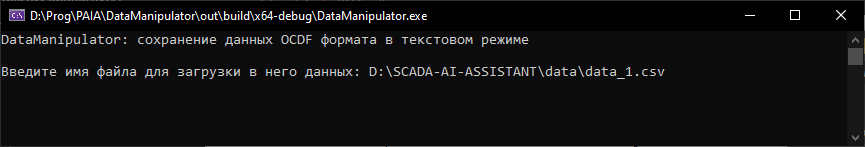
\includegraphics[width=\textwidth]{images/forDataManipulator/OCDFsafeCSV.png}
    \caption{сохранение OCDF-данных в текстовом режиме.}
    \label{fig:OCDFsafeCSV}
  \end{figure}

  \par Из особенностей, хотелось бы отметить, что при сохранении в текстовом режиме требуется обязательно указывать расширение файла, поскольку текстово можно сохранить в любом формате, кроме зарезервированных форматов. Но всё же рекомендуется указывать расширение .csv.
}

\subsubsection{ \standartTitleFont
  Сохранение OCDF-данных в бинарный файл.
} \label{subsubsec:OCDFSafeBIN}

{\standartFont

  \par Для сохранения данных в бинарном режиме нужно выбрать соответствующий пункт меню и в появившемся запросе указать путь к файлу, в который будут сохранены данные. Это продемонстрировано на рисунке \ref{fig:OCDFsafeBIN}.

  \begin{figure}[H]
    \centering
    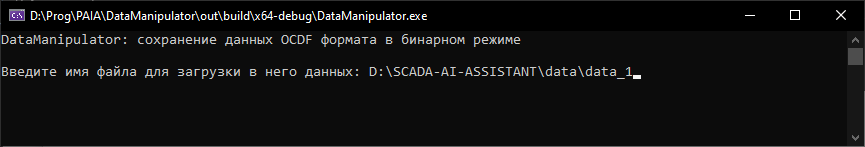
\includegraphics[width=\textwidth]{images/forDataManipulator/OCDFsafeBIN.png}
    \caption{сохранение OCDF-данных в бинарном режиме.} 
    \label{fig:OCDFsafeBIN}
  \end{figure}

  \par Из особенностей, хотелось бы отметить, что при сохранении в бинарном режиме не обязательно указывать расширение файла, поскольку расширение .bin будет добавлено автоматически, даже если расширение указать. 
}

\subsubsection{ \standartTitleFont
  Возможные ошибки при сохранении OCDF-данных в файл.
} \label{subsubsec:OCDFSageErr}

{\standartFont

  \par В качестве ошибок может выступать ввод зарезервированных форматов при сохранении в текстовом режиме, таких как .tlstm, .vlstm, .lstm, .bin, что показано на рисунке \ref{fig:OCDFsafeERes}.

  \begin{figure}[H]
    \centering
    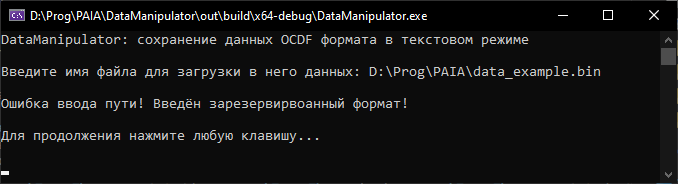
\includegraphics[width=\textwidth]{images/forDataManipulator/OCDFsafeCSVErrReser.png}
    \caption{сохранение OCDF-данных в бинарном режиме.}
    \label{fig:OCDFsafeERes}
  \end{figure}

  \par также к ошибкам можно отнести слишком маленькое имя файла. Имя файла должно иметь более 5 символов в своём названии включая расширение. Эта ошибка продемонстрирована на рисунке \ref{fig:OCDFsafeEInv}.

  \begin{figure}[H]
    \centering
    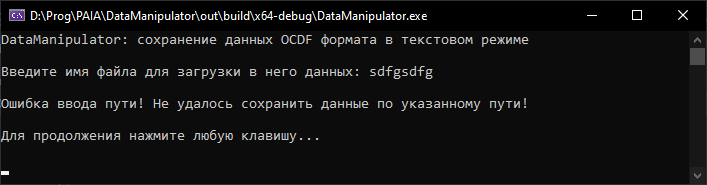
\includegraphics[width=\textwidth]{images/forDataManipulator/OCDFsafeCSVErrInvalid.png}
    \caption{сохранение OCDF-данных в бинарном режиме.}
    \label{fig:OCDFsafeEInv}
  \end{figure}
}

\subsection{ \standartTitleFont
  Выход из меню работы с OCDF-данными.
} \label{subsec:OCDFOut}

{\standartFont

  \par Для выхода из меню работы с OCDF-данными достаточно ввести 0 и тогда загруженные из файла OCDF-данные освободятся из памяти, поэтому перед выходом из меню не забудьте сохранить результаты обработки данных.

  \par
}

\subsection{ \standartTitleFont
  Визуализация TDF-данных.
} \label{subsubsec:TDFVisual}

{\standartFont

  \par Для визуализации данных нужно выбрать соответствующий пункт меню и дождаться появления окна с визуализированными данными. Вводить ничего не требуется.

  \par TDF-данные содержат информацию всех сидов, поэтому будет построено 6 графиков для каждого сида. Вся информация о сидах будет содержаться в легенде. Визуализация TDF-данных представлена на рисунке \ref{fig:TDFVisual}.

  \begin{figure}[H]
    \centering
    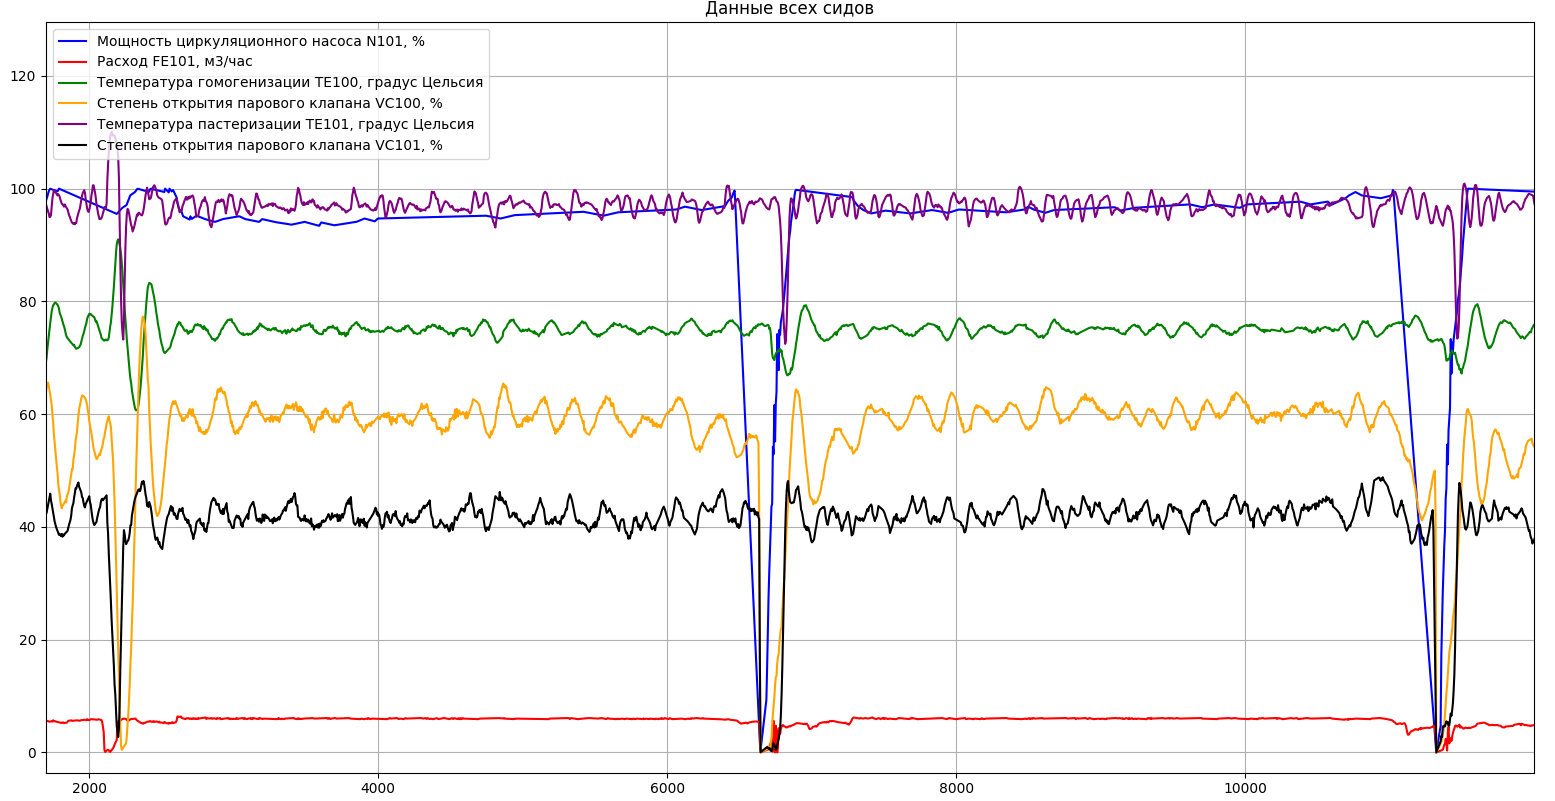
\includegraphics[width=\textwidth]{images/forDataManipulator/TDFVisual.png}
    \caption{пример визуализации TDF-данных}
    \label{fig:TDFVisual}
  \end{figure}

  \par Масштабирование графиков описано в разделе \ref{subsubsec:OCDFVisualControl}.

  \par Управление перейдёт к основной программе только после закрытия окна визуализации.

  \par
}

\subsection{ \standartTitleFont
  Сохранение TDF-данных в файл.
} \label{subsec:TDFSafe}

{\standartFont

  \par После работы с данными конечно же появится надобность в сохранении результатов обработки данных. Для этого есть возможность сохранить данные в текстовом или бинарном режимах.

  \par Возможные ошибки при сохранении данных, которые могут возникать, уже описаны в разделе \ref{subsubsec:OCDFSageErr}.

  \par
}

\subsubsection{ \standartTitleFont
  Сохранение TDF-данных в файл формата csv.
} \label{subsubsec:TDFSafeCSV}

{\standartFont

  \par Для сохранения TDF-данных в текстовом режиме достаточно выбрать соответствующий пункт меню и в появившемся запросе указать путь к файлу, в который будут сохранены данные. Это продемонстрировано на рисунке \ref{fig:TDFsafeCSV}.

  \begin{figure}[H]
    \centering
    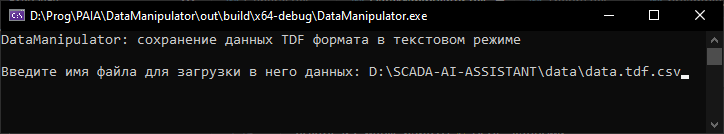
\includegraphics[width=\textwidth]{images/forDataManipulator/TDFsafeCSV.png}
    \caption{сохранение TDF-данных в текстовом режиме.}
    \label{fig:TDFsafeCSV}
  \end{figure}

  \par Из особенностей, хотелось бы отметить, что при сохранении в текстовом режиме требуется обязательно указывать расширение файла, поскольку текстово можно сохранить в любом формате, кроме зарезервированных форматов. Но всё же рекомендуется указывать расширение .csv.
}

\subsubsection{ \standartTitleFont
  Сохранение TDF-данных в бинарный файл.
} \label{subsubsec:TDFSafeBIN}

{\standartFont

  \par Для сохранения TDF-данных в бинарном режиме достаточно выбрать соответствующий пункт меню и в появившемся запросе указать путь к файлу, в который будут сохранены данные. Это продемонстрировано на рисунке \ref{fig:TDFsafeBIN}.

  \begin{figure}[H]
    \centering
    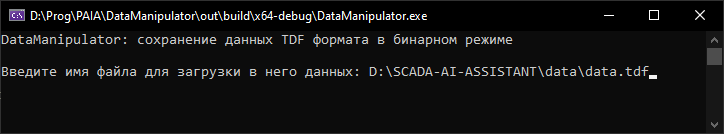
\includegraphics[width=\textwidth]{images/forDataManipulator/TDFsafeBIN.png}
    \caption{сохранение TDF-данных в бинарном режиме.}
    \label{fig:TDFsafeBIN}
  \end{figure}

  \par Из особенностей, хотелось бы отметить, что при сохранении в бинарном режиме не обязательно указывать расширение файла, поскольку расширение .bin будет добавлено автоматически, даже если расширение указать.
}

\subsection{ \standartTitleFont
  Выход из меню работы с TDF-данными.
} \label{subsubsec:TDFOut}

{\standartFont

  \par Для выхода из меню работы с TDF-данными достаточно ввести 0 и тогда загруженные из файла TDF-данные освободятся из памяти, поэтому перед выходом из меню не забудьте сохранить результаты обработки данных.

  \par
}

\subsection{ \standartTitleFont
  Создание TDF-данных.
} \label{subsubsec:CreateTDF}

\subsubsection{ \standartTitleFont
  Смысл TDF-данных.
} \label{subsubsec:CreateTDFTarget}

{\standartFont

  \par TDF-данные {--} это аккуратные данные, представленные в одной таблице, где имеется информация о всех сидах в определённый момент времени. TDF-данные нужны по большей мере для визуализации, а также дальнейшего парсинга на OCDF-данные, поскольку из TDF-данных очень удобно и надёжно можно получать хорошие наборы данных для обучения.

  \par
}

\subsubsection{ \standartTitleFont
  Механизм построения TDF-данных.
} \label{subsubsec:CreateTDFHow}

{\standartFont

  \par Сперва необходимо загрузить файл с OCDF-данными, который содержал бы все сиды. После этого идёт процесс парсинга данных, который описан в разделе \ref{subsec:OCDFPars}, в ходе которого создаются 6 последовательностей данных, каждая из которых характеризует свой сид. Пример продемонстрирован на рисунке \ref{fig:CreateTDFstage1}, где указаны всего 3 последовательности данных, чтобы не нагружать пример, а над ячейками последовательности указаны некоторые моменты времени.

  \begin{figure}[H]
    \centering
    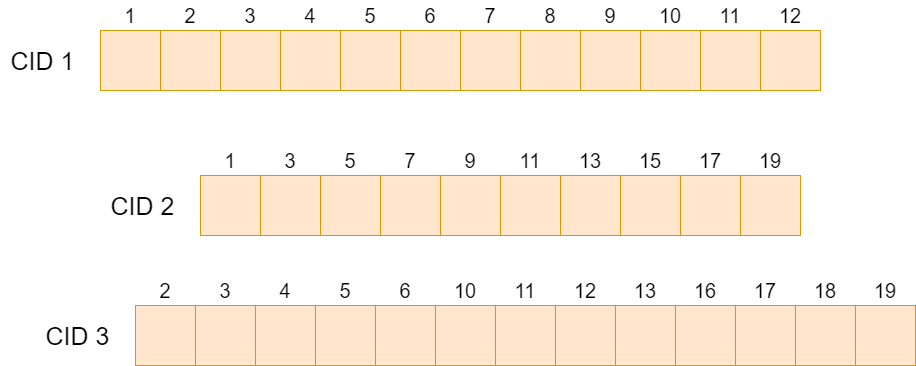
\includegraphics[width=\textwidth]{images/forDataManipulator/CreateTDFstage1.drawio.png}
    \caption{пример последовательностей данных для сборки TDF-данных.}
    \label{fig:CreateTDFstage1}
  \end{figure}

  \par Как видно из рисунка, в большинстве случаев значения различных сидов будут определены не во все моменты времени, что недопустимо для TDF-данных. Это необходимо решить.

  \par Пользователю предоставляется возможность ввести временной интервал между соседними точками для будущих TDF-данных. Этот процесс является процессом выравнивания диапазонов для OCDF-данных, который уже описан в разделе \ref{subsec:OCDFRightIntervals}.

  \par Но перед превращением каждой последовательности в равноинтервальные данные, требуется определить стартовые и конечные границы. Для определения стартовой границы берутся первые элементы всех последовательностей и среди них отбирается самый поздний по времени момент. Этот элемент на рисунке \ref{fig:CreateTDFstage2} закрашен синим цветом. Далее проверяется, есть ли определённое значение в других последовательностях данных в этот момент времени. Если да, то работа идёт дальше, если нет, то это значение определяется по правилам, описанным в разделе \ref{subsubsec:OCDFRIMath}. Появившиеся элементы на рисунке \ref{fig:CreateTDFstage2} изображены зелёным цветом. Элементы, идущие раньше него по времени удаляются из всех последовательностей данных. Удалённые данные на рисунке \ref{fig:CreateTDFstage2} закрашены красным цветом. Для определения конечной границы берутся последние элементы всех последовательностей и среди них отбирается самый ранний по времени момент. Этот элемент на рискунке \ref{fig:CreateTDFstage2} закрашен синим цветом. Далее проверяется, есть ли определённое значение в других последовательностях данных в этот момент времени. Если да, то работа идёт дальше, если нет, то это значение определяется по правилам, описанным в разделе \ref{subsubsec:OCDFRIMath}. Элементы, идущие позже него по времени удаляются из всех последовательностей данных. Удалённые данные на рисунке \ref{fig:CreateTDFstage2} закрашены красным цветом.

  \begin{figure}[H]
    \centering
    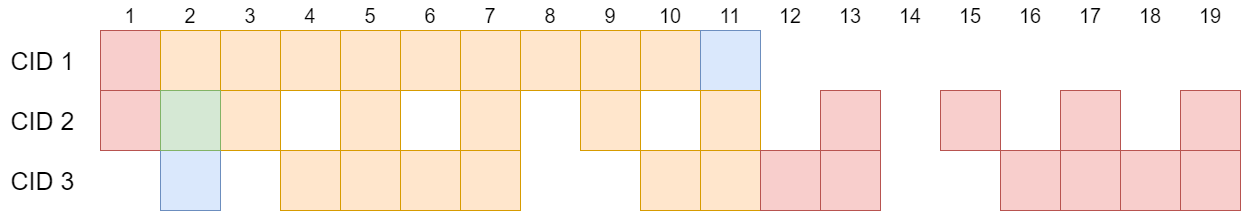
\includegraphics[width=\textwidth]{images/forDataManipulator/CreateTDFstage2.drawio.png}
    \caption{обработка последовательностей данных для сборки TDF-данных.}
    \label{fig:CreateTDFstage2}
  \end{figure}

  \par После этой операции происходит процесс выравнивания диапазонов. Для примера интервал будет составлять 1. На рисунке \ref{fig:CreateTDFstage3} добавленные элементы таким образом закрашены зелёным цветом.

  \begin{figure}[H]
    \centering
    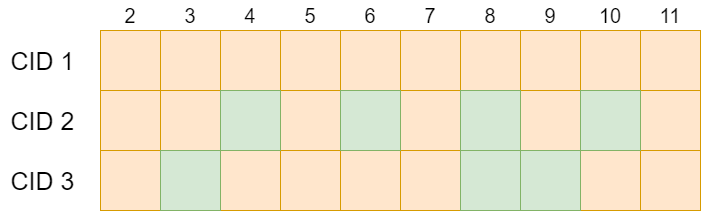
\includegraphics[width=\textwidth]{images/forDataManipulator/CreateTDFstage3.drawio.png}
    \caption{привидение к единообразию по времени последовательностей OCDF-данных.}
    \label{fig:CreateTDFstage3}
  \end{figure}

  \par в конечном итоге все последовательности данных записываются в вектор TDF-данных, где ключевым полем будет время, а значение сидов в любой из этих моментов времени будет определён. По сути один любой столбец на рисунке \ref{fig:CreateTDFstage3} обозначает строку TDF-данных, но только с 6-ю сидами.

}

\subsubsection{ \standartTitleFont
  Процесс построения TDF-данных.
} \label{subsubsec:CreateTDFProc}

{\standartFont

  \par При построении TDF-данных сперва будет предложено ввести имя файла с данных, содержащие в себе информацию о всех сидах в формате OCDF. Процесс чтения данных уже рассмотрен в разделе \ref{subsubsec:ReadOCDF} и продемонстрирован на рисунке \ref{fig:CreateTDFReadData}.

  \begin{figure}[H]
    \centering
    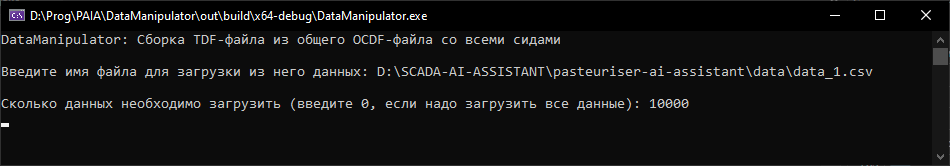
\includegraphics[width=\textwidth]{images/forDataManipulator/CreateTDFReadData.png}
    \caption{считывание OCDF-данных для сборки TDF-данных.}
    \label{fig:CreateTDFReadData}
  \end{figure}

  \par После будет предложено ввести будущий интервал между соседними точками для достижения равноинтервальных TDF-данных. Процесс выравнивания диапазонов уже рассмотрен в разделе \ref{subsec:OCDFRightIntervals} и продемонстрирован на рисунке \ref{fig:CreateTDFRI}.

  \begin{figure}[H]
    \centering
    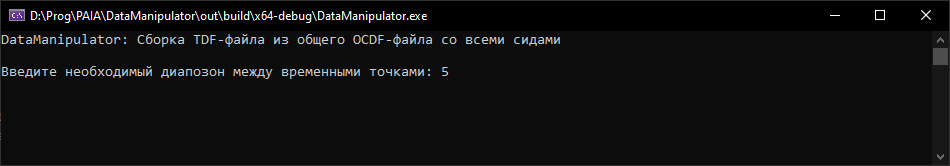
\includegraphics[width=\textwidth]{images/forDataManipulator/CreateTDFRI.png}
    \caption{ввод интервала между соседними точками в TDF-данных.}
    \label{fig:CreateTDFRI}
  \end{figure}

  \par После этого начинают происходить процессы, описанные в разделе выше. После их завершения будет предложено ввести имя файла, для сохранения получившихся табличных данных, они же TDF-данные, что продемонстрировано на рисунке \ref{fig:CreateTDFSR}.

  \begin{figure}[H]
    \centering
    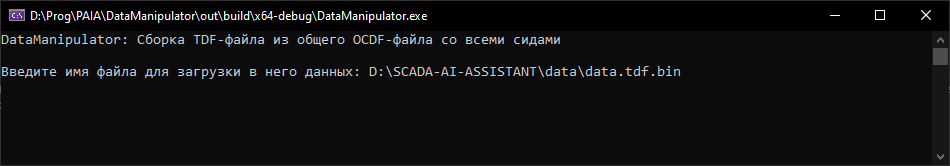
\includegraphics[width=\textwidth]{images/forDataManipulator/CreateTDFSafeResult.png}
    \caption{сохранение собранных TDF-данных.}
    \label{fig:CreateTDFSR}
  \end{figure}

  \par При вводе имени файла нет никаких ограничений. Из рекомендаций есть только то, что при вводе имени файла лучше указать расширение .tdf, чтобы различать файлы с TDF-данными.
  
  \par После ввода имени файла будет предложено выбрать режим сохранения: текстовым иди бинарный режим, введя 0 или 1, соответственно. Это продемонстрировано на рисунке \ref{fig:CreateTDFTS}.

  \begin{figure}[H]
    \centering
    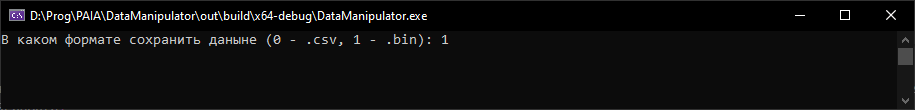
\includegraphics[width=\textwidth]{images/forDataManipulator/CreateTDFTypeSafe.png}
    \caption{выбор режима сохранения собранных TDF-данных.}
    \label{fig:CreateTDFTS}
  \end{figure}

  \par На этом процесс построения TDF-данных завершается.

  \par 

}

\subsubsection{ \standartTitleFont
  Возможные ошибки при построении TDF-данных.
} \label{subsubsec:CreateTDFErr}

{\standartFont

  \par Поскольку в данной операции имеет место быть чтение OCDF-данных из файла, то и ошибки она имеет соответствующие, которые уже разобраны в разделе \ref{subsubsec:ReadOCDF}.

  \par Также при сборке TDF-данных используется и операция выравнивания диапазонов по оси X, возможные ошибки которой описаны в разделе \ref{subsubsec:OCDFRIErr}.

  \par Теперь разберём специфические ошибки, которые встречаются только при сборке TDF-данных. Основной ошибкой является отсутствие хотя бы одного сида в загруженных данных. Если нет информации о каком-либо сиде, то TDF-данные построить невозможно. Эта ошибка продемонстрирована на рисунке \ref{fig:CreateTDFErr1}.

  \begin{figure}[H]
    \centering
    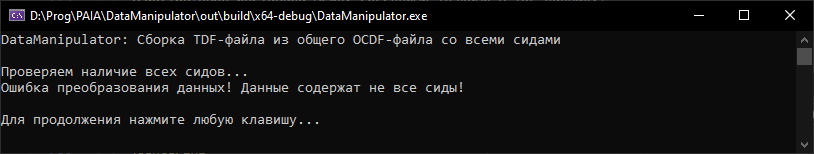
\includegraphics[width=\textwidth]{images/forDataManipulator/CreateTDFErr1.png}
    \caption{ошибка нехватки сидов в OCDF-данных.}
    \label{fig:CreateTDFErr1}
  \end{figure}

  \par Также формирование TDF-данных невозможно, если у какого-либо сида менее трёх примеров данных по одному сиду. Такая ошибка продемонстрирована на рисунке \ref{fig:CreateTDFErr2}.

  \begin{figure}[H]
    \centering
    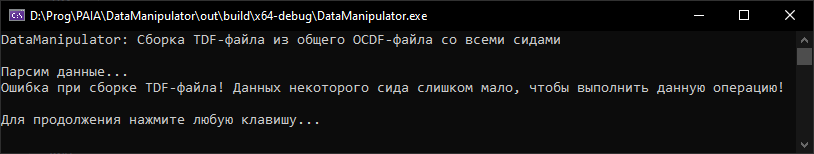
\includegraphics[width=\textwidth]{images/forDataManipulator/CreateTDFErr2.png}
    \caption{малое количество данных некоторого сида при сборке TDF-данных.}
    \label{fig:CreateTDFErr2}
  \end{figure}

  \par При выборе режима сохранения: текстовом или бинарном - ошибкой будет ввод отличных от 0 или 1 символов.

  \par
}
